\documentclass{article}
\usepackage{graphicx} %
\usepackage{tikz}
\usepackage{amsmath}
\usepackage{amssymb}
\usepackage{graphicx}
\usepackage{multicol}
\graphicspath{ {./img/} }
\usetikzlibrary{arrows}

\title{Kalkulus 1 Latihan Soal 2.4}
\author{Gilbran Mahdavikia Raja}
\date{5025241134}

\begin{document}

\begin{flushleft}
    Gilbran Mahdavikia Raja \\
    5025241134 \\
\end{flushleft}
\begin{description}
    \item[$1.$] Diberikan suatu fungsi $f(x)=2+\sqrt{x-1}$ dan garis $l$ yang melalui titik $(1,2)$ dan $(7,5)$. 
    \begin{description}
        \item[$(a)$] Buatlah sketsa kurva $f(x)$ dan garis $l$
        \item[] \begin{enumerate} 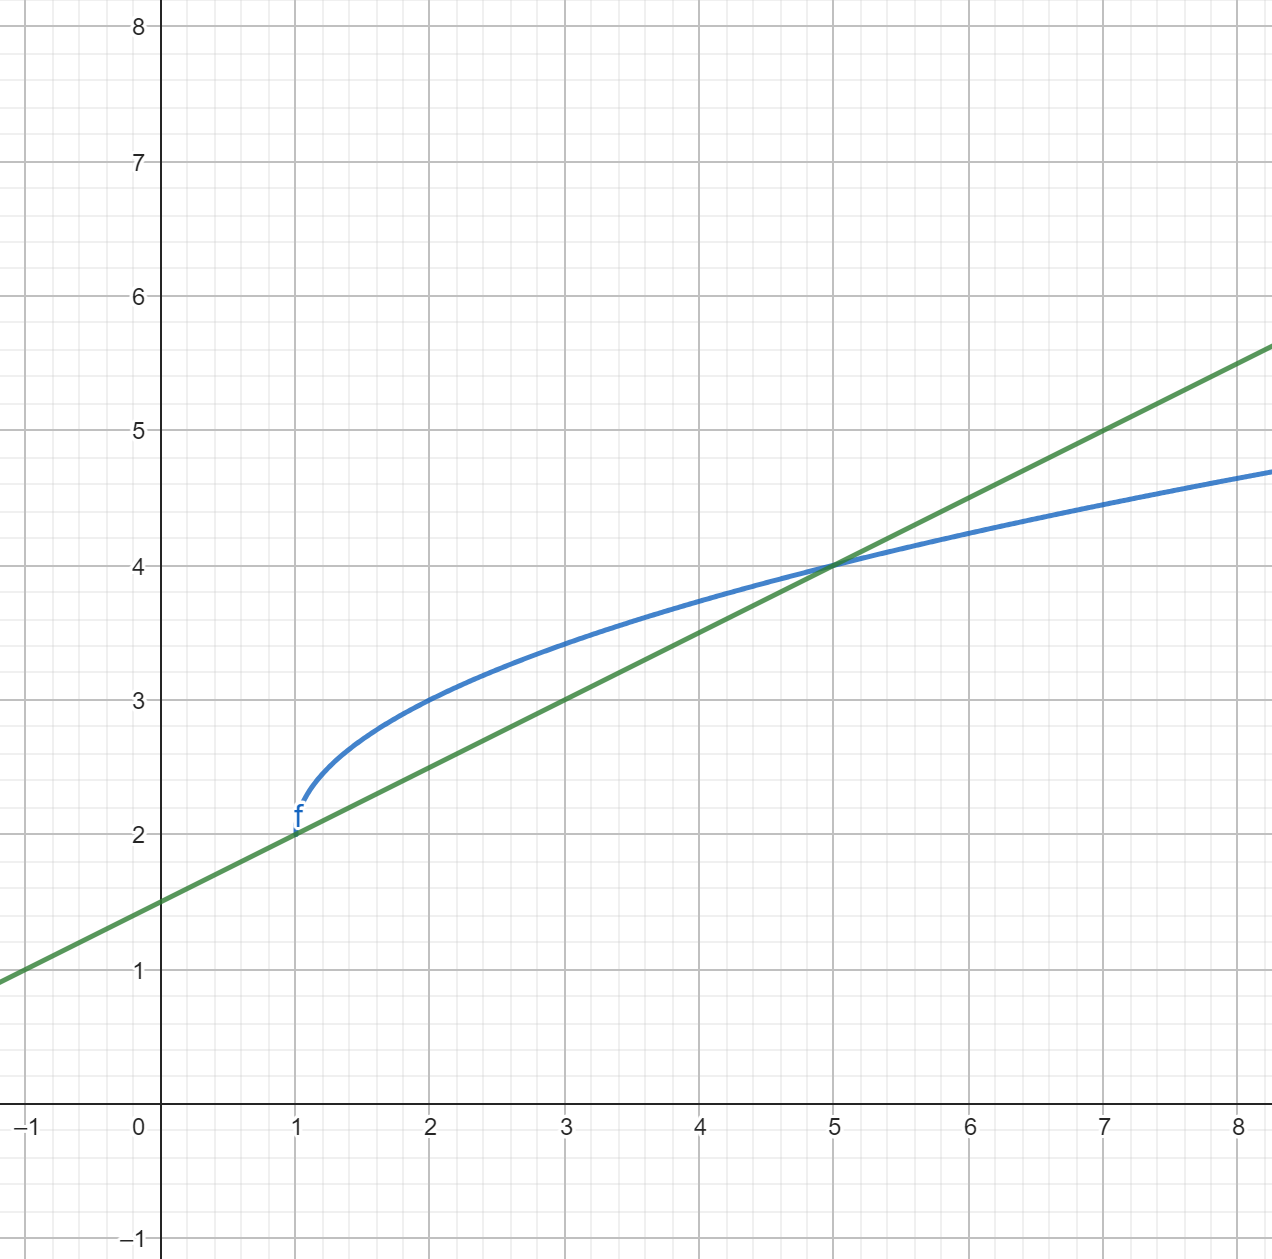
\includegraphics[scale=0.17]{1.png}\end{enumerate}
        \item[$(b)$] Tentukan titik potong antara kurva $f(x)$ dan garis $l$ 
        \begin{description}
            \item[$\Leftrightarrow$] $ml = \frac{5-2}{7-1}$
            \item[$\Leftrightarrow$] $ml = \frac{1}{2}$
            \item[$\Leftrightarrow$] $l \rightarrow y-2=\frac{1}{2}(x-1)$
            \item[$\Leftrightarrow$] $l \rightarrow y=\frac{x+3}{2}$
            \item[$\Leftrightarrow$] $2+\sqrt{x-1} = \frac{x+3}{2}$
            \item[$\Leftrightarrow$] $4 +2\sqrt{x-1} = x+3$
            \item[$\Leftrightarrow$] $2\sqrt{x-1} = x-1$
            \item[$\Leftrightarrow$] $\sqrt{x-1} = \frac{x}{2}-\frac{1}{2}$
            \item[$\Leftrightarrow$] $x-1 = \frac{(x-1)^2}{4}$
            \item[$\Leftrightarrow$] $x=1 \cup x = 5 \\ y = 2 \cup y = 4$
            \item[$\Leftrightarrow$] titik potong antara kurva $f(x)$ dan garis $l = (1,2),(5,4)$
        \end{description}
    \end{description}
    \item[$2.$] Diberikan fungsi $f(x)=a+\sqrt{x-b}$ dan $g(x)=(x-a)^2+b$
    \begin{description}
        \item[$(a)$] Tentukan domain dan range $f(x)$
        \begin{description}
            \item[$\Leftrightarrow$] $\mathcal{D}f = [b,+\infty)$
            \item[$\Leftrightarrow$] $\mathcal{R}f = [a,+\infty)$
        \end{description}
        \item[$(b)$] Tentukan domain $g(x)$, agar fungsi $f(x)$ dan $g(x)$ saling invers.
        \begin{description}
            \item[$\Leftrightarrow$] $\mathcal{D}g = [a,+\infty)$
        \end{description}
    \pagebreak
    \item[$(c)$]sketsa kurva $f(x)$ dan $f^-1$ dalam suatu bidang koordinat\\(a = 3, b = 4)
    \item[] \begin{enumerate} 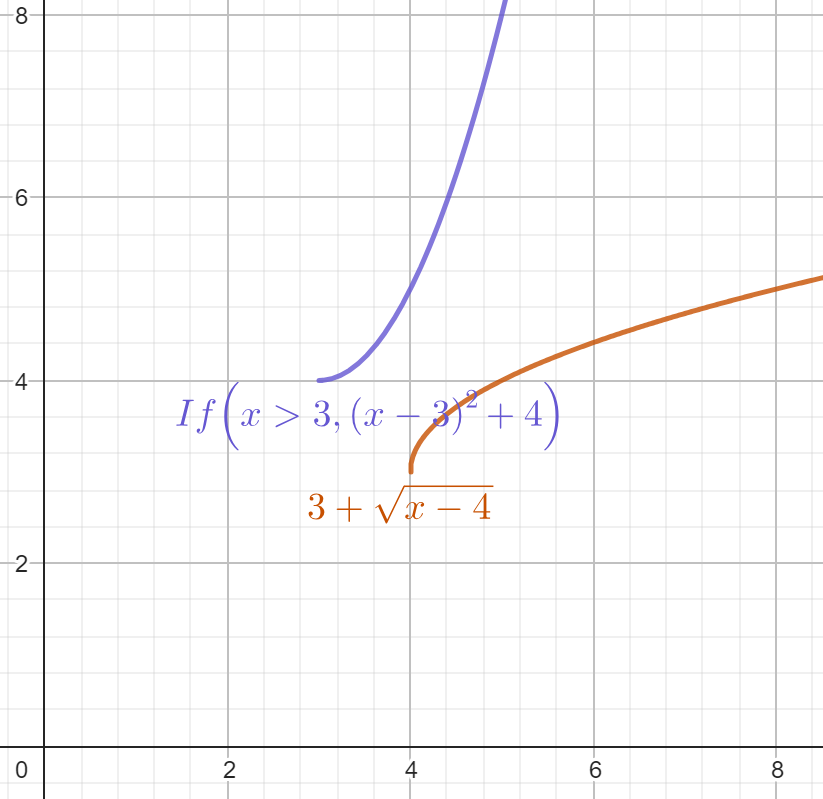
\includegraphics[scale=0.25]{2.png}\end{enumerate}
    \end{description}
    \item[$3.$]$g(x)$ =  $\left\{ \begin{array}{rcl}
        (px)^2 & \mbox{,} & x \leq 2 \\ 
        (x+p) & \mbox{,} & x > 2 \\
        \end{array}\right.$ \\
    Nilai $p$ yang mungkin agar $g(x)$ kontinu \\
    lim$_{x\rightarrow2^-} g(x) =$  lim$_{x\rightarrow2^+} g(x)$ \\
    $\Leftrightarrow$ lim$_{x\rightarrow2^-} (px)^2$ =  lim$_{x\rightarrow2^+} (x+p)$ \\
    $\Leftrightarrow (2p)^2 = 2 + p$  \\
    $\Leftrightarrow 4p^2 - p -2 = 0$  \\
    Jadi $p = \frac{1 \pm \sqrt{33}}{8}$ \\
    Jadi, agar $g(x)$ kontinu, nilai $p = \frac{1 + \sqrt{33}}{8}$ atau $p = \frac{1 - \sqrt{33}}{8}$
    \item[$4.$] Tentukan semua nilai $x$ yang memenuhi $|2x-1| + x = |x-2| + 3$
    \begin{description}
        \item[] $|2x-1|$ =  $\left\{ \begin{array}{rcl}
        2x-1 & \mbox{,} & x \geq -\frac{1}{2} \\ 
        -2x+1 & \mbox{,} & x < -\frac{1}{2} \\
        \end{array}\right.$
        \item[] $|x-2|$ =  $\left\{ \begin{array}{rcl}
        x-2 & \mbox{,} & x \geq 2 \\ 
        -x+2 & \mbox{,} & x < 2 \\
        \end{array}\right.$ \\
    \end{description}

    untuk $x < -\frac{1}{2}$
    \begin{description}
        \item[$\Leftrightarrow$] $-2x-1+x = (-x+2) + 3$ 
        \item[$\Leftrightarrow$] $-x-1 = -x+5$ 
        \item[$\Leftrightarrow$] $0 = 6$ (Tidak memenuhi)
    \end{description}
    untuk $-\frac{1}{2} \leq x < 2$
    \begin{description}
        \item[$\Leftrightarrow$] $2x+1+x = (-x+2) + 3$ 
        \item[$\Leftrightarrow$] $3x+1= -x + 5$ 
        \item[$\Leftrightarrow$] $4x= 4$ (Tidak memenuhi)
        \item[$\Leftrightarrow$] $x= 1$ (Tidak memenuhi)
    \end{description}
    untuk $x \geq 2$ \\ 
    \begin{description}
        \item[$\Leftrightarrow$] $2x+1+x = (x-2)+3$ 
        \item[$\Leftrightarrow$] $3x+1= x+1$ 
        \item[$\Leftrightarrow$] $2x= 0$
        \item[$\Leftrightarrow$] $x= 0$ (Tidak memenuhi)
        \item[] Jadi penyelesaiannya adalah $x = 1$ 
    \end{description}

    \item $f(x) = \frac{x^3 + x^2 + x - 3}{x-1}$ 
    \begin{description}
        \item[$\Leftrightarrow$]lim$_{x\rightarrow1} f(x)$ 
        \item[$\Leftrightarrow$] lim$_{x\rightarrow1} \frac{x^3 + x^2 + x - 3}{x-1}$ 
        \item[$\Leftrightarrow$] lim$_{x\rightarrow1} \frac{(x-1)(x^2+2x+3)}{x-1}$ 
        \item[$\Leftrightarrow$] lim$_{x\rightarrow1} (x^2+2x+3)$ 
        \item[$\Leftrightarrow$] 6
    \end{description}
\end{description}

\end{document}